\documentclass[aspectratio=169]{beamer}
\usetheme{simple}

\input{preamble/preamble.tex}
\input{preamble/preamble_math.tex}
% \input{preamble/preamble_acronyms.tex}

\title{Hidden Markov Models}
\subtitle{STATS 305B: Applied Statistics}
\author{Scott Linderman}
\date{\today}

\date{\today}


\begin{document}


\maketitle


\begin{frame}{Recap}

    Last time...
    \begin{itemize}
        \item Mixture Models (Gaussian and general exp-fam)
        \item K-Means as MAP estimation
        \item EM as maximizing the marginal log likelihood
        \item Connecting EM and VI
    \end{itemize}
    
\end{frame}
    
    
\begin{frame}{Outline}
    
    Today...
    \begin{itemize}
        \item Hidden Markov Models
        \item The forward-backward algorithm
        \item EM for HMMs
        \item Implementation Details
    \end{itemize}
    
\end{frame}
    

\begin{frame}{Recap: Gaussian Mixture Models}
Recall the basic Gaussian mixture model,
\begin{align}
    z_t &\iid{\sim} \mathrm{Cat}(\mbpi) \\
    x_t \mid z_t &\sim \cN(\mbmu_{z_t}, \mbSigma_{z_t})
\end{align}
where 
\begin{itemize}
    \item $z_t \in \{1,\ldots,K\}$ is a \textbf{latent mixture assignment}
    \item $x_t \in \reals^D$ is an \textbf{observed data point}
    \item $\mbpi \in \Delta_K$, $\mbmu_k \in \reals^D$, and $\mbSigma_k \in \reals_{\succeq 0}^{D \times D}$ are parameters
\end{itemize}
(Here we've switched to indexing data points by $t$ rather than $n$.)

Let $\mbTheta$ denote the set of parameters. We can be Bayesian and put a prior on $\mbTheta$ and run Gibbs or VI, or we can point estimate $\mbTheta$ with EM, etc.
\end{frame}


\begin{frame}[t]{Recap: Gaussian Mixture Models II}
\textbf{Draw the graphical model.}
% We can write the joint distribution as,
% \begin{align}
%     p(\mbz_{1:T}, \mbx_{1:T}; \mbTheta) &= \prod_{t=1}^T p(z_t; \mbTheta) \, p(\mbx_t \mid z_t, \mbTheta).
% \end{align}
% Or we can group terms differently,
% \begin{align}
%     p(\mbz_{1:T}, \mbx_{1:T}; \mbTheta) 
%     &= \left[ \prod_{t=1}^T p(z_t; \mbTheta) \right] \left[ \prod_{t=1}^T p(\mbx_t \mid z_t, \mbTheta) \right] \\
%     &= p(\mbz_{1:T}) p(\mbx_{1:T} \mid \mbz_{1:T})
% \end{align}
% From this perspective, we 
\end{frame}


\begin{frame}[t]{Recap: Gaussian Mixture Models III}
Recall the EM algorithm for mixture models,
\begin{itemize}
    \item \textbf{E step: } Compute the posterior distribution 
    \begin{align}
        q(\mbz_{1:T}) 
        &= p(\mbz_{1:T} \mid \mbx_{1:T}; \mbTheta) \\
        &= \prod_{t=1}^T p(z_t \mid \mbx_t; \mbTheta) \\
        &= \prod_{t=1}^T q_t(z_t)
    \end{align}
    \item \textbf{M step: } Maximize the ELBO wrt $\mbTheta$,
    \begin{align}
        \cL(\mbTheta) 
        &= \E_{q(\mbz_{1:T})}\left[\log p(\mbx_{1:T}, \mbz_{1:T}; \mbTheta) - \log q(\mbz_{1:T}) \right] \\
        &= \E_{q(\mbz_{1:T})}\left[\log p(\mbx_{1:T}, \mbz_{1:T}; \mbTheta) \right]  + c.
    \end{align}
\end{itemize}
For exponential family mixture models, the M-step only requires expected sufficient statistics.
\end{frame}


\begin{frame}{Hidden Markov Models}
Hidden Markov Models (HMMs) are like mixture models with temporal dependencies between the mixture assignments.

\begin{center}
    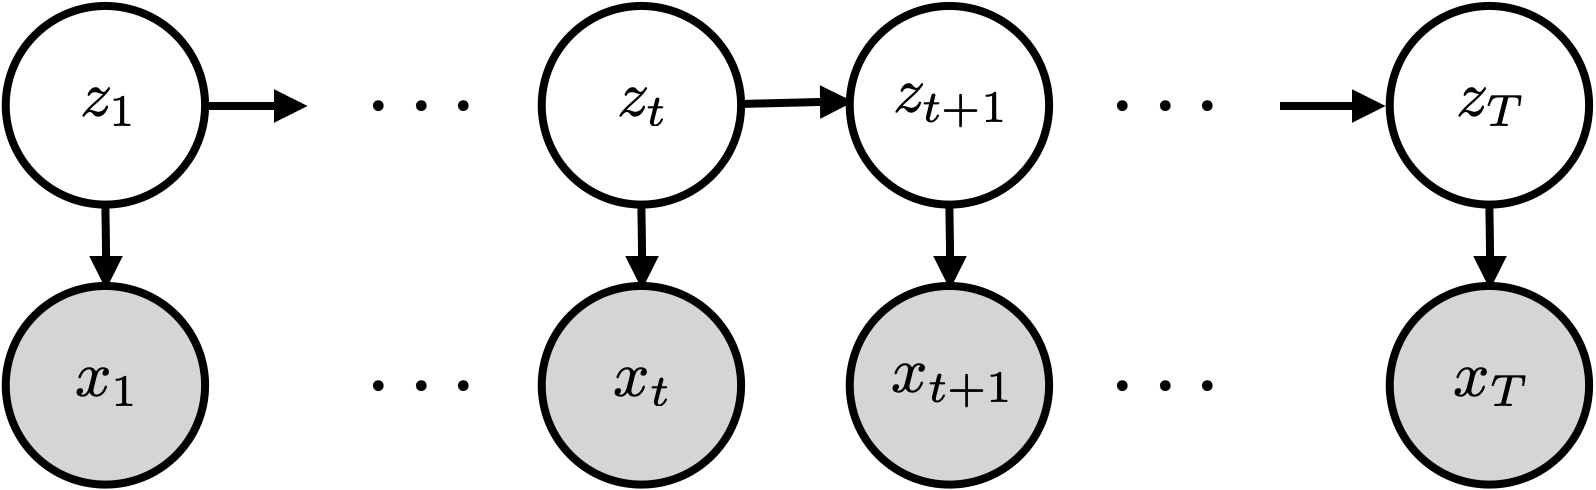
\includegraphics[width=0.7\textwidth]{11_hmms/hmm.png}    
\end{center}

This graphical model says that the joint distribution factors as,
\begin{align}
    p(z_{1:T}, \mbx_{1:T}) &= p(z_1) \prod_{t=2}^T p(z_t \mid z_{t-1}) \prod_{t=1}^T p(\mbx_t \mid z_t).
\end{align}
We call this an HMM because the \textit{hidden} states follow a Markov chain, $p(z_1) \prod_{t=2}^T p(z_t \mid z_{t-1})$.
\end{frame}

\begin{frame}{Hidden Markov Models II}
An HMM consists of three components:
\begin{enumerate}
    \item \textbf{Initial distribution:} $z_1 \sim \mathrm{Cat}(\mbpi_0)$ 
    \item \textbf{Transition matrix:} $z_t \sim \mathrm{Cat}(\mbP_{z_{t-1}})$ where $\mbP \in [0,1]^{K \times K}$ is a \textit{row-stochastic} transition matrix with rows $\mbP_k$.
    \item \textbf{Emission distribution:} $\mbx_t \sim p(\cdot \mid \mbtheta_{z_t})$
\end{enumerate}
\end{frame}

\begin{frame}{Example: The \emph{occasionally} dishonest casino}
    \begin{figure}
        \centering
        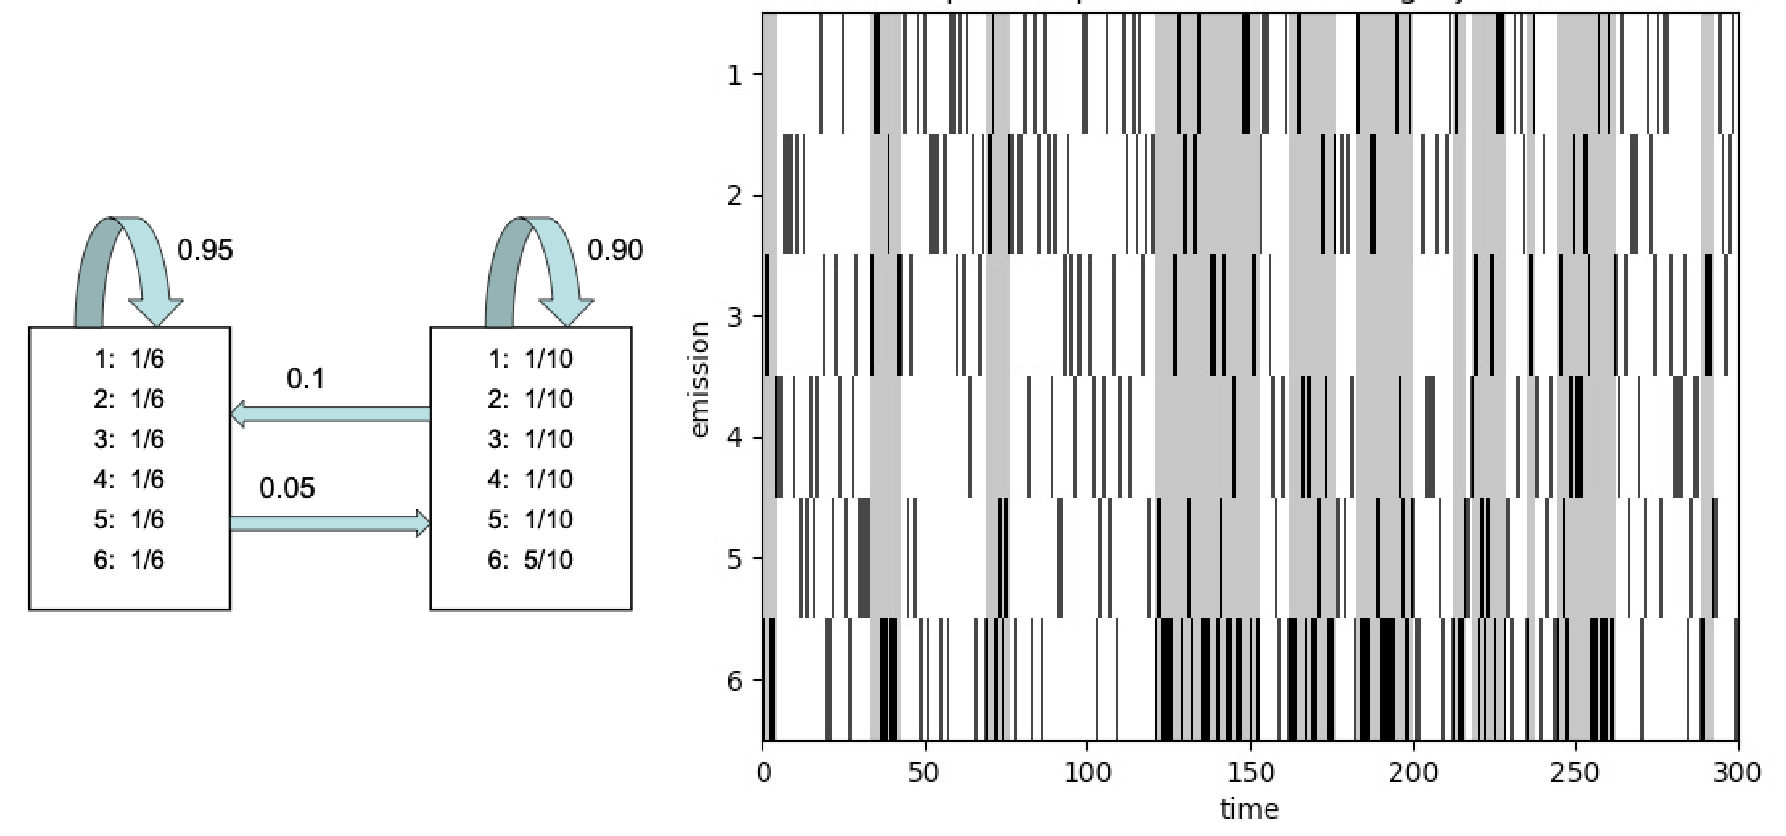
\includegraphics[width=5in]{11_hmms/dishonest_casino.png}
        \caption{An \emph{occasionally} dishonest casino that sometimes throws loaded dice. From~\url{https://probml.github.io/dynamax/notebooks/hmm/casino_hmm_inference.html}}
        \label{fig:casino}
    \end{figure}
\end{frame}

\begin{frame}{Example: HMM for splice site recognition}
    \begin{figure}
        \centering
        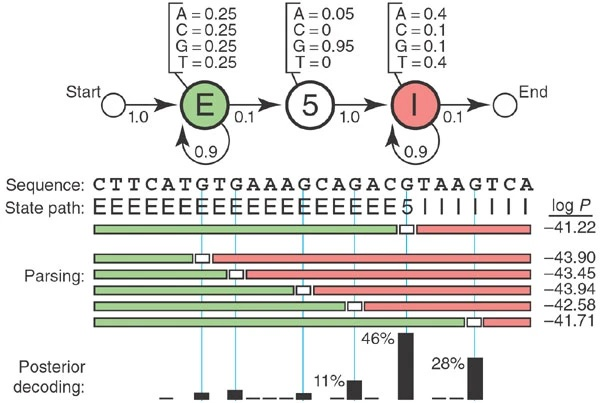
\includegraphics[width=3.5in]{11_hmms/hmm_genome.jpg}
        \caption{A toy model for parsing a genome to find 5' splice sites. From~\citet{eddy2004hidden}.}
        \label{fig:genome}
    \end{figure}
    \vspace{-1em}
    \textbf{Question:} Suppose the splice site always had a \texttt{GT} sequence. How would you change the model to detect such sites?
\end{frame}

\begin{frame}{Example: Autoregressive HMM for video segmentation}

    \vspace{1em}
    \begin{figure}
        \centering
        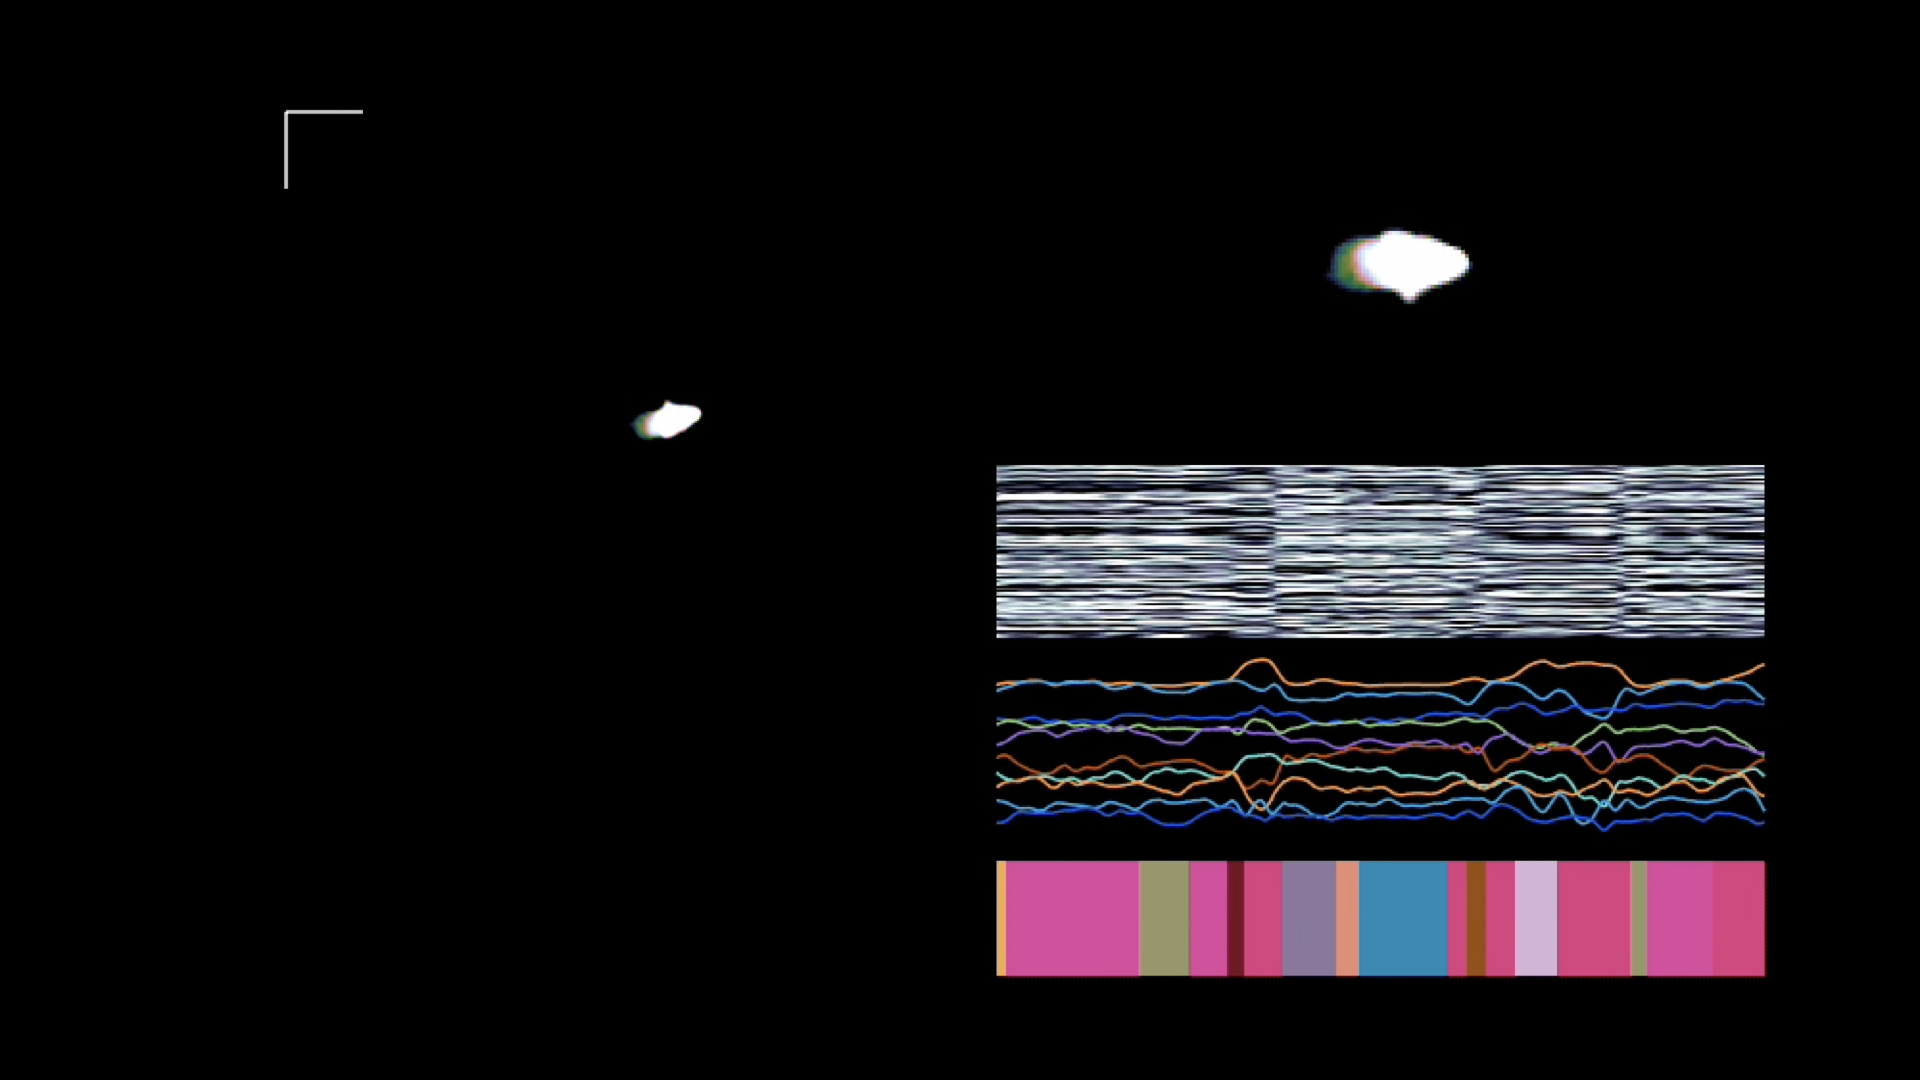
\includegraphics[width=4.75in]{11_hmms/moseq.png}
        \caption{Segmenting videos of freely moving mice~\citep{wiltschko2015mapping}. (Show video.)}
        \label{fig:moseq}
    \end{figure}
\end{frame}

\begin{frame}{Hidden Markov Models III}
We are interested in questions like:
\begin{itemize}
    % \item What are the \textit{filtering distributions} of $p(z_{t} \mid \mbx_{1:t})$?
    \item What are the \textit{predictive distributions} of $p(z_{t+1} \mid \mbx_{1:t})$?
    \item What is the \textit{posterior marginal} distribution $p(z_t \mid \mbx_{1:T})$?
    \item What is the \textit{posterior pairwise marginal} distribution $p(z_t, z_{t+1} \mid \mbx_{1:T})$?
    \item What is the \textit{posterior mode} $z_{1:T}^\star = \argmax p(z_{1:T} \mid \mbx_{1:T})$?
    \item How can we \textit{sample the posterior} $p(\mbz_{1:T} \mid \mbx_{1:T})$ of an HMM?
    \item What is the \textit{marginal likelihood} $p(\mbx_{1:T})$?
    \item How can we \textit{learn the parameters} of an HMM?
\end{itemize}
\textbf{Question:} Why might these sound like hard problems?
\end{frame}

% \begin{frame}{Computing the filtering distributions}
%     The filtering distributions give the probability of the latent state $z_t$ given observations \textit{up to and including} time $t$.
%     \begin{align}
%         p(z_t \mid \mbx_{1:t}) 
%         &= \sum_{z_1=1}^K \cdots \sum_{z_{t-1}=1}^K \prod_{s=1}^{t} p(z_s \mid z_{s-1}) \, p(\mbx_s \mid z_s) \\
%         &= \sum_{z_{t-1}=1}^K \left[ \left( \sum_{z_1=1}^K \cdots \sum_{z_{t-2}=1}^K \prod_{s=1}^{t-1} p(z_s \mid z_{s-1}) \, p(\mbx_s \mid z_s) \right) p(z_t \mid z_{t-1}) \, p(x_t \mid z_t) \right]  \\
%         &= \sum_{z_{t-1}=1}^K \left[ p(\mbz_{t-1} \mid \mbx_{1:t-1}) \, p(z_t \mid z_{t-1}) \, p(x_t \mid z_t) \right] 
%     \end{align}
% \end{frame}

\begin{frame}{Computing the predictive distributions}
    The predictive distributions give the probability of the latent state $z_{t+1}$ given observations \textit{up to but not including} time $t+1$.
    Let,
    \begin{align}
        \alpha_{t+1}(z_{t+1}) &\triangleq p(z_{t+1}, \mbx_{1:t}) \\
        &= \sum_{z_1=1}^K \cdots \sum_{z_{t}=1}^K p(z_1) \prod_{s=1}^{t} p(\mbx_s \mid z_s) \, p(z_{s+1} \mid z_{s})\\
        &= \sum_{z_{t}=1}^K \left[ \left( \sum_{z_1=1}^K \cdots \sum_{z_{t-1}=1}^K p(z_1) \prod_{s=1}^{t-1} p(\mbx_s \mid z_s) \, p(z_{s+1} \mid z_{s}) \right) p(\mbx_t \mid z_t) \, p(z_{t+1} \mid z_{t}) \right]  \\
        &= \sum_{z_{t}=1}^K \alpha_t(z_t) \, p(\mbx_t \mid z_t) \, p(z_{t+1} \mid z_{t}).
    \end{align}
    We call $\alpha_t(z_t)$ the \textit{forward messages}. 
    We can compute them recursively! The base case is $p(z_1 \mid \varnothing) \triangleq p(z_1)$.
\end{frame}


\begin{frame}{Computing the predictive distributions II }
    We can also write these recursions in a vectorized form. Let 
    \begin{align}
        \mbalpha_t &= 
        \begin{bmatrix}
        \alpha_t(z_t = 1) \\
        \vdots \\
        \alpha_t(z_t=K)
        \end{bmatrix}
        =
        \begin{bmatrix}
        p(z_t = 1, \mbx_{1:t-1}) \\
        \vdots \\
        p(z_t = K, \mbx_{1:t-1})
        \end{bmatrix}
        \qquad \text{and} \qquad
        \mbl_t = 
        \begin{bmatrix}
        p(\mbx_t \mid z_t = 1) \\
        \vdots \\
        p(\mbx_t \mid z_t = K)
        \end{bmatrix}
    \end{align}
    both be vectors in $\reals_+^K$. Then,
    \begin{align}
        \mbalpha_{t+1} &= \mbP^\top (\mbalpha_t \odot \mbl_t)
    \end{align}
    where $\odot$ denotes the Hadamard (elementwise) product and $\mbP$ is the transition matrix.
\end{frame}

\begin{frame}[t]{Computing the predictive distributions III}
    Finally, to get the predictive distributions we just have to normalize,
    \begin{align}
        p(z_{t+1} \mid \mbx_{1:t}) &\propto p(z_{t+1}, \mbx_{1:t}) = \alpha_{t+1}(z_{t+1}).
    \end{align}
    \textbf{Question:} What does the normalizing constant tell us?
\end{frame}

\begin{frame}{Computing the posterior marginal distributions}
    The posterior marginal distributions give the probability of the latent state $z_{t}$ given \textit{all the observations} up to time $T$.
    \begin{align}
        p(z_{t} \mid \mbx_{1:T}) 
        &= \sum_{z_1=1}^K \cdots \sum_{z_{t-1}=1}^K \sum_{z_{t+1}=1}^K \cdots \sum_{z_T=1}^K p(\mbz_{1:T}, \mbx_{1:T}) \\
        &= \nonumber 
        \bigg[ \sum_{z_{t}=1}^K \cdots \sum_{z_{t-1}=1}^K p(z_1) \prod_{s=1}^{t-1} p(\mbx_s \mid z_s) \, p(z_{s+1} \mid z_{s}) \bigg]
        \times  p(\mbx_t \mid z_t)   \\
        &\qquad \times \bigg[ \sum_{z_{t+1}=1}^K \cdots \sum_{z_T=1}^K \prod_{u=t+1}^T p(z_{u} \mid z_{u-1}) \, p(\mbx_u \mid z_u) \bigg] \\
        &= \alpha_t(z_t) \times p(\mbx_t \mid z_t) \times \beta_t(z_t)
    \end{align}
    where we have introduced the \textit{backward messages} $\beta_t(z_t)$.
\end{frame}

\begin{frame}{Computing the backward messages}
    The backward messages can be computed recursively too,
    \begin{align}
        \beta_t(z_t) 
        &\triangleq \sum_{z_{t+1}=1}^K \cdots \sum_{z_T=1}^K \prod_{u=t+1}^T p(z_{u} \mid z_{u-1}) \, p(\mbx_u \mid z_u) \\
        &= \sum_{z_{t+1}=1}^K p(z_{t+1} \mid z_t) \, p(\mbx_{t_1} \mid z_{t+1}) \left(\sum_{z_{t+2}=1}^K \cdots \sum_{z_T=1}^K \prod_{u=t+2}^T p(z_{u} \mid z_{u-1}) \, p(\mbx_u \mid z_u) \right) \\
        &= \sum_{z_{t+1}=1}^K p(z_{t+1} \mid z_t) \, p(\mbx_{t_1} \mid z_{t+1}) \, \beta_{t+1}(z_{t+1}).
    \end{align}
    For the base case, let $\beta_T(z_T) = 1$.
\end{frame}

\begin{frame}{Computing the backward messages (vectorized)}
    Let 
    \begin{align}
        \mbbeta_t &= 
        \begin{bmatrix}
        \beta_t(z_t = 1) \\
        \vdots \\
        \beta_t(z_t=K)
        \end{bmatrix}
    \end{align}
    be a vector in $\reals_+^K$. Then,
    \begin{align}
        \mbbeta_{t} &= \mbP (\mbbeta_{t+1} \odot \mbl_{t+1}).
    \end{align}
    Let $\mbbeta_T = \mbone_K$.
    
    Now we have everything we need to compute the posterior marginal,
    \begin{align}
        p(z_t = k \mid \mbx_{1:T}) &= \frac{\alpha_{t,k} \, l_{t,k} \, \beta_{t,k}}{\sum_{j=1}^K \alpha_{t,j} l_{t,j} \beta_{t,j}}.
    \end{align}
    
    We just derived the \textbf{forward-backward algorithm} for HMMs~\citep{rabiner1986introduction}.
\end{frame}

\begin{frame}[t]{What do the backward messages represent?}
\textbf{Question:} If the forward messages represent the predictive probabilities $\alpha_{t+1}(z_{t+1}) = p(z_{t+1}, \mbx_{1:t})$, what do the backward messages represent?
\end{frame}

\begin{frame}[t]{Computing the posterior pairwise marginals}
\textbf{Exercise:} Use the forward and backward messages to compute the posterior pairwise marginals $p(z_t, z_{t+1} \mid \mbx_{1:T})$.
\end{frame}

% \begin{frame}[t]{Computing the marginal likelihood}
% EM maximizes the marginal likelihood by iteratively constructing and maximizing a lower bound. How can we compute the marginal likelihood and track our progress?

% Start by applying the chain rule:
% \begin{align}
%     p(\mbx_{1:T}) 
%     &= \prod_{t=1}^T p(\mbx_t \mid \mbx_{1:t-1}) \\
%     &= \prod_{t=1}^T \sum_{z_t=1}^K p(z_t \mid \mbx_{1:t-1}) p(\mbx_t \mid z_t) \\
%     &= \prod_{t=1}^T \sum_{k=1}^K \alpha_{t,k} \, l_{t,k}
% \end{align}

% \end{frame}

\begin{frame}{Normalizing the messages for numerical stability}
    If you're working with long time series, especially if you're working with 32-bit floating point, you need to be careful. 
    
    The messages involve products of probabilities, which can quickly overflow. 
    
    There's a simple fix though: after each step, re-normalize the messages so that they sum to one. I.e replace
    \begin{align}
        \mbalpha_{t+1} &= \mbP^\top (\mbalpha_t \odot \mbl_t)
    \end{align}
    with 
    \begin{align}
        \widetilde{\mbalpha}_{t+1} &= \frac{1}{A_t} \mbP^\top (\widetilde{\mbalpha}_t \odot \mbl_t) \\
        A_t &= \sum_{k=1}^K \sum_{j=1}^K P_{jk} \widetilde{\alpha}_{t,j} l_{t,j}
            \equiv \sum_{j=1}^K \widetilde{\alpha}_{t,j} l_{t,j} \quad \text{(since $\mbP$ is row-stochastic)}.
    \end{align}
    This leads to a nice interpretation: The normalized messages are predictive likelihoods $\widetilde{\alpha}_{t+1,k} = p(z_{t+1}=k \mid \mbx_{1:t})$, and the normalizing constants are $A_t = p(\mbx_t \mid \mbx_{1:t-1})$.
\end{frame}

\begin{frame}{EM for Hidden Markov Models}
Now we can put it all together. To perform EM in an HMM,
\begin{itemize}
    \item \textbf{E step: } Compute the posterior distribution 
    \begin{align}
        q(\mbz_{1:T}) 
        &= p(\mbz_{1:T} \mid \mbx_{1:T}; \mbTheta).
    \end{align}
    (Really, run the \textbf{forward-backward algorithm} to get posterior marginals and pairwise marginals.)
    
    \item \textbf{M step: } Maximize the ELBO wrt $\mbTheta$,
    \begin{align}
        \cL(\mbTheta) 
        &= \E_{q(\mbz_{1:T})}\left[\log p(\mbx_{1:T}, \mbz_{1:T}; \mbTheta) \right]  + c \\
        &= \nonumber \E_{q(\mbz_{1:T})}\left[\sum_{k=1}^K \mathbb{I}[z_1=k]\log \pi_{0,k} \right] + 
        \E_{q(\mbz_{1:T})}\left[\sum_{t=1}^{T-1} \sum_{i=1}^K \sum_{j=1}^K \mathbb{I}[z_t=i, z_{t+1}=j]\log P_{i,j} \right] \\
        &\qquad + \E_{q(\mbz_{1:T})}\left[\sum_{t=1}^T \sum_{k=1}^K \mathbb{I}[z_t=k]\log p(\mbx_t; \theta_k) \right] 
    \end{align}
\end{itemize}
For exponential family observations, the M-step only requires expected sufficient statistics.
\end{frame}

\begin{frame}{What else?}
    \begin{itemize}
        \item How can we sample the posterior?
        \item How can we find the posterior mode?
        \item How can we choose the number of states?
        \item What if my transition matrix is sparse?
    \end{itemize}
\end{frame}



\begin{frame}[t,allowframebreaks]
        \frametitle{References}
        \bibliographystyle{unsrtnat}
        \bibliography{refs.bib}
\end{frame}

\end{document}